\documentclass[xcolor=table]{beamer}

% \rowcolors{1}{gray!30}{gray!10}

\usetheme{Boadilla}
\usecolortheme{dolphin}
\useoutertheme[subsection=false]{smoothbars}

\setbeamercolor{frametitle}{fg = black, bg = white} 
\setbeamercolor{palette primary}{use=structure,fg=white,bg=structure.fg!60!white}
\setbeamercolor{palette secondary}{use=structure,fg=white,bg=structure.fg!90!white}
\setbeamercolor{palette tertiary}{use=structure,fg=white,bg=structure.fg!120!white}
\setbeamercolor{palette quaternary}{use=structure,fg=black,bg=white} %Top bar

\setbeamertemplate{enumerate subitem}[circle]%
\renewcommand{\insertsubenumlabel}{\alph{enumii}}

\usepackage{amsmath}
\usepackage{xcolor}
\usepackage{booktabs}
\usepackage[utf8]{inputenc}
\usepackage{hyperref}
\usepackage[table]{xcolor}
\usepackage{setspace}
\usepackage{parskip}

\definecolor{lightgray}{gray}{0.9}

\hypersetup{
    colorlinks,
    citecolor=blue,
    linkcolor=blue
}

\usepackage{listings} %include R code

\definecolor{codegreen}{rgb}{0,0.6,0}
\definecolor{codegray}{rgb}{0.5,0.5,0.5}
\definecolor{codepurple}{rgb}{0.58,0,0.82}
\definecolor{backcolour}{rgb}{0.95,0.95,0.92}

\lstdefinestyle{mystyle}{
    backgroundcolor=\color{backcolour},   
    commentstyle=\color{codegreen},
    keywordstyle=\color{magenta},
    numberstyle=\tiny\color{codegray},
    stringstyle=\color{codepurple},
    basicstyle=\ttfamily\tiny,
    breakatwhitespace=false,         
    breaklines=true,                 
    captionpos=b,                    
    keepspaces=true,                 
    numbers=left,                    
    numbersep=5pt,                  
    showspaces=false,                
    showstringspaces=false,
    showtabs=false,                 
    columns=fullflexible,
    frame=single,
    tabsize=2
}

\lstset{style=mystyle}


\author{Jonathan P. Latner, PhD}
\title{Best practices for creating synthetic data: Balancing efficiency, utility, and privacy}
\date{\today}

\beamertemplatenavigationsymbolsempty 
\setbeamerfont{page number in head/foot}{size=\tiny}
\setbeamertemplate{footline}[frame number]
\setbeamertemplate{caption}[numbered]
\setbeamertemplate{section in toc}[sections numbered]

\begin{document}

\section{Introduction}\label{sec:intro}
\frame{\frametitle{ }
\titlepage
\thispagestyle{empty}
}

\frame{\frametitle{What is synthetic data?}
\begin{itemize}
    \scriptsize
    \item `When Rubin (1993) introduced the idea of fully synthetic data, there was considerable appeal to releasing data that represented ``no actual individual's'' responses, and skepticism regarding its feasability.  Subsequent research has adequately demonstrated the feasibility.  However the basic question ``How much protection does synthetic data methodology provide?'' remained largely unanswered.' (Abowd \& Vilhuber, 2008)
    \item `The idea of synthetic data sets is similar.  A statistical process is used to extract information from an actual set collected from a set of respondents and is reexpressed as  a collection of artificial or synthetic data sets for public consumption.  This allows wide dissemination of the informational content of the actual data set and, at the same time, limits the exposure to potential inadvertent of malicious disclosure of sensitive information about the respondents.' (Raghunathan, 2021)
    \item A promising alternative to address the trade-off between broad data access and disclosure protection is the release of synthetic data.  With this approach, {\bf a model is fitted to the original data and draws from this model are used to replace the original values.}  Depending on the desired level of protection, only some records (partial synthesis) or the entire dataset (full synthesis) are replaced by synthetic values. (Drechsler \& Haensch, 2023)
\end{itemize}
}

\frame{\frametitle{What are the trade-offs when creating synthetic data?}
\begin{itemize}
    \item Privacy (risk) vs. utility
    \begin{itemize}
        \item How do we measure privacy?
        \item How do we measure utility?
    \end{itemize}
    \item Computational efficiency (duration in time)
    \begin{itemize}
        \item It takes a long time!
        \item Role of hyperparameters results in better output, but takes even longer
    \end{itemize}
    \item Methods vs. packages 
    \begin{itemize}
        \item Does the package do what it says (Synthpop)?
        \item Is the package the best version of the method (CTGAN)?
    \end{itemize}
\end{itemize}
}

\frame{\frametitle{Balancing risk vs. utility}
\begin{figure}
    \caption{Little et al., 2022 (WP), Table 2}
    \resizebox{\textwidth}{!}{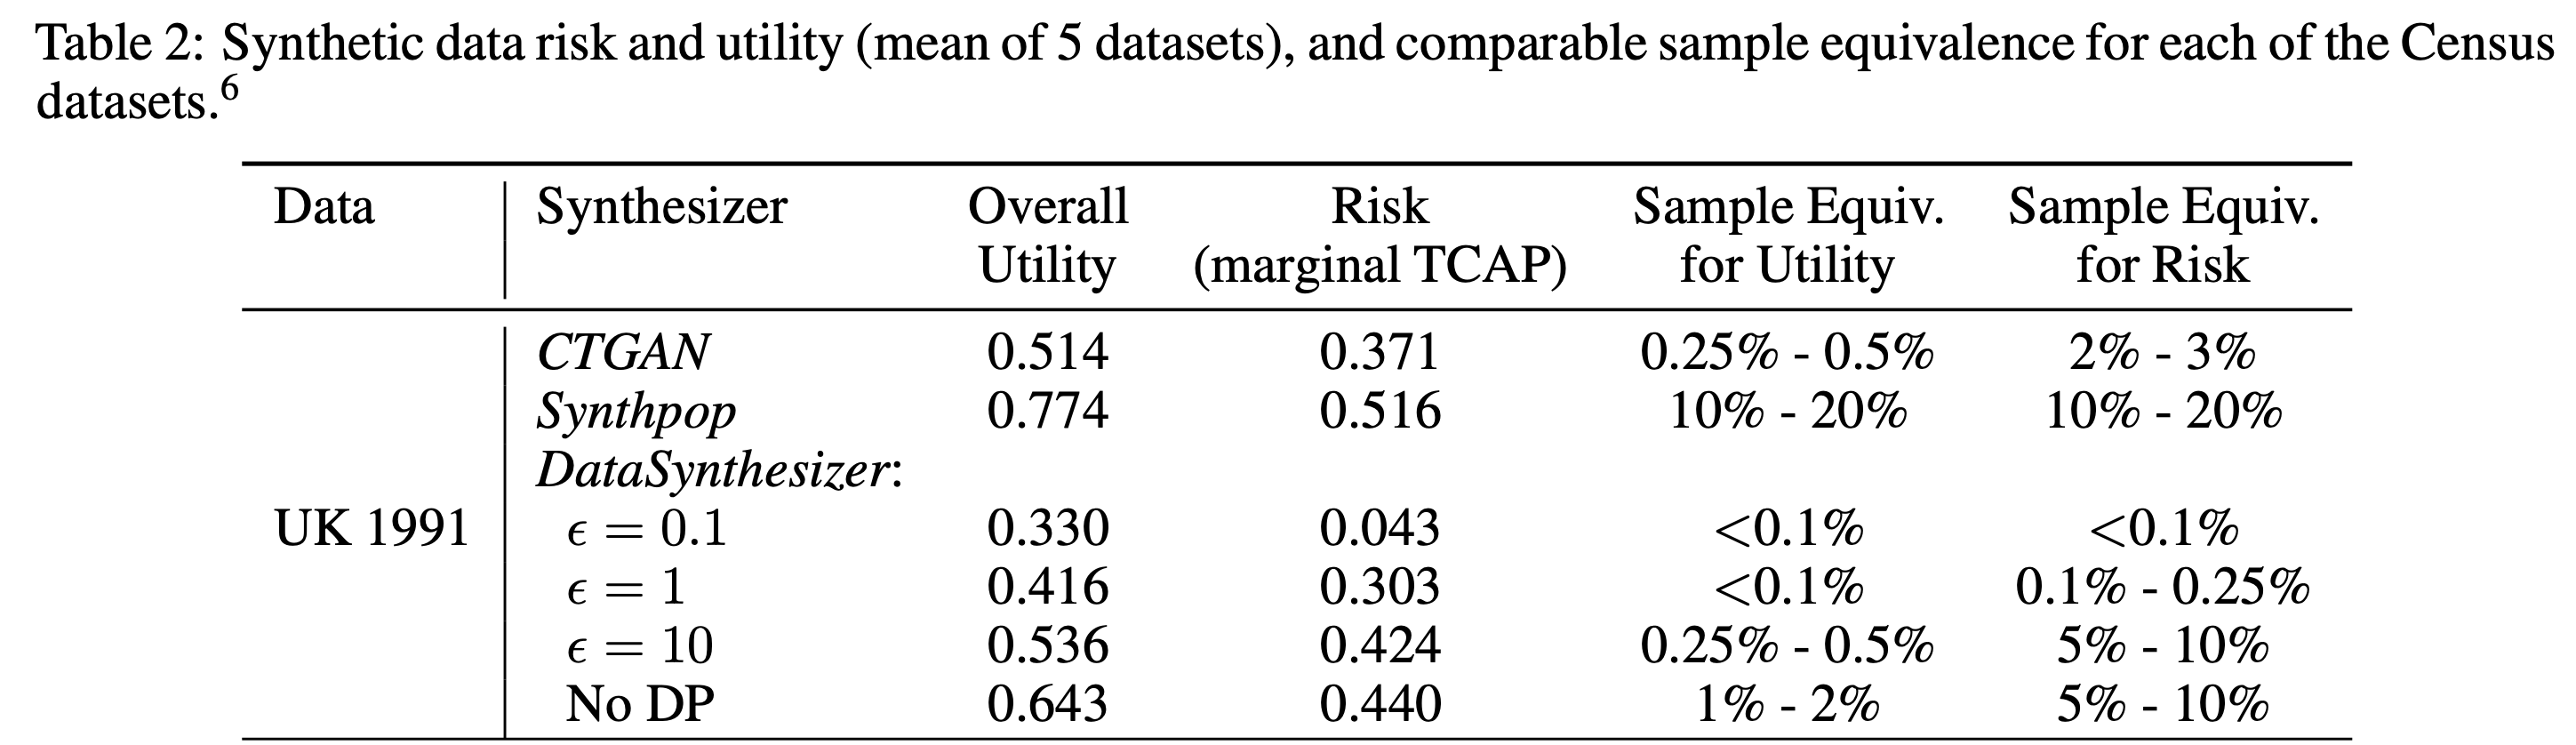
\includegraphics{../support_files/little_etal_2022_table_2.png}}
    \label{}
\end{figure}

Key finding: Synthpop is clear `winner', with highest utility and risk, equivalent to releasing a 10-20\% sample
}

\frame{\frametitle{Data dimensions}
\begin{table}[!h]
    \caption{JPL replication of UK 1991}
    \centering
    \resizebox{.9\textwidth}{!}{% latex table generated in R 4.3.0 by xtable 1.8-4 package
% Fri Nov 17 14:30:19 2023
\begin{tabular}{lrrrr}
  \toprule
Data & Rows & Columns & NumericVars & NonNumericVars \\ 
  \midrule
adult & 32561 &  15 &   6 &   9 \\ 
  df\_ods & 200000 &  20 &  20 &   0 \\ 
  grid & 20000 &   2 &   2 &   0 \\ 
  gridr & 20000 &   2 &   2 &   0 \\ 
  sd2011 & 5000 &  35 &  14 &  21 \\ 
  sd2011\_small & 5000 &   4 &   2 &   2 \\ 
  sim\_categorical1 & 1000 &  10 &   0 &  10 \\ 
  sim\_categorical10 & 1000 &  20 &   0 &  20 \\ 
  sim\_categorical11 & 1000 &  20 &   0 &  20 \\ 
  sim\_categorical12 & 1000 &  20 &   0 &  20 \\ 
  sim\_categorical13 & 5000 &  10 &   0 &  10 \\ 
  sim\_categorical14 & 5000 &  10 &   0 &  10 \\ 
  sim\_categorical15 & 5000 &  10 &   0 &  10 \\ 
  sim\_categorical16 & 5000 &  10 &   0 &  10 \\ 
  sim\_categorical17 & 5000 &  15 &   0 &  15 \\ 
  sim\_categorical18 & 5000 &  15 &   0 &  15 \\ 
  sim\_categorical19 & 5000 &  15 &   0 &  15 \\ 
  sim\_categorical2 & 1000 &  10 &   0 &  10 \\ 
  sim\_categorical20 & 5000 &  15 &   0 &  15 \\ 
  sim\_categorical21 & 5000 &  20 &   0 &  20 \\ 
  sim\_categorical22 & 5000 &  20 &   0 &  20 \\ 
  sim\_categorical23 & 5000 &  20 &   0 &  20 \\ 
  sim\_categorical24 & 5000 &  20 &   0 &  20 \\ 
  sim\_categorical3 & 1000 &  10 &   0 &  10 \\ 
  sim\_categorical4 & 1000 &  10 &   0 &  10 \\ 
  sim\_categorical5 & 1000 &  15 &   0 &  15 \\ 
  sim\_categorical6 & 1000 &  15 &   0 &  15 \\ 
  sim\_categorical7 & 1000 &  15 &   0 &  15 \\ 
  sim\_categorical8 & 1000 &  15 &   0 &  15 \\ 
  sim\_categorical9 & 1000 &  20 &   0 &  20 \\ 
  sim\_continuous\_1 & 50000 &  10 &  10 &   0 \\ 
  sim\_continuous\_2 & 50000 &  15 &  15 &   0 \\ 
  sim\_continuous\_3 & 50000 &  20 &  20 &   0 \\ 
  sim\_continuous\_4 & 100000 &  10 &  10 &   0 \\ 
  sim\_continuous\_5 & 100000 &  15 &  15 &   0 \\ 
  sim\_continuous\_6 & 100000 &  20 &  20 &   0 \\ 
  sim\_continuous\_7 & 200000 &  10 &  10 &   0 \\ 
  sim\_continuous\_8 & 200000 &  15 &  15 &   0 \\ 
  sim\_continuous\_9 & 200000 &  20 &  20 &   0 \\ 
   \bottomrule
\end{tabular}
}
    \label{}
\end{table}
\begin{figure}
    \caption{Little et al., 2022 (WP), Table 1}
    \vskip -5mm
    \resizebox{\textwidth}{!}{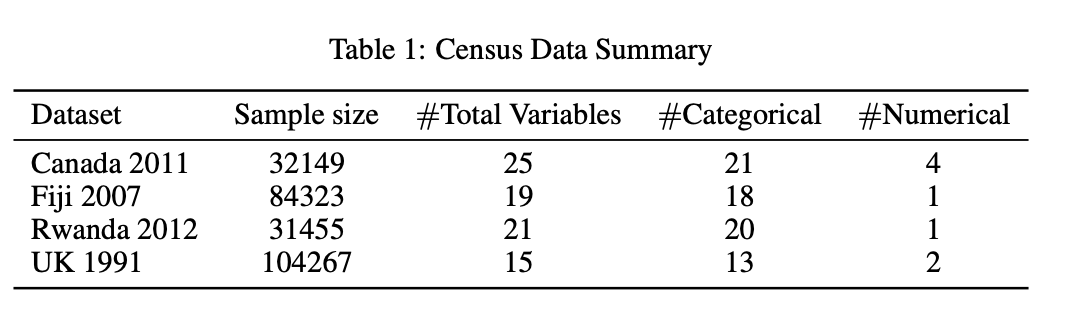
\includegraphics{../support_files/little_etal_2022_table_1.png}}
    \label{}
\end{figure}
}

\frame{\frametitle{Duration in time (UK 1991)}
\begin{figure}
    \caption{}
    \resizebox{\textwidth}{!}{\includegraphics{"/Users/jonathanlatner/Google Drive/My Drive/IAB/little_etal_2021/graphs/graph_compare_duration.pdf"}}
    \label{}
\end{figure}
}

\frame{\frametitle{Whats the problem?}
\begin{enumerate}
    \item All data sets are low dimensional (rows, obs, variable type)
    \item Privacy and utility overlap (TCAP/CIO from 1 regression)
    \begin{itemize}
        \item Disadvantage: 1 regression seems limited
        \item Advantage: Are more regressions better?
        \item Other measure of utility is ROC (univ + bivar)
    \end{itemize}
    \item Synthpop is compared to Datasynthesizer and CTGAN using baseline hyperparameters
    \begin{itemize}
        \item Not comparing apples to apples
    \end{itemize}
    \item {\bf Synthpop appears to be the best, but this is a function of research choice (data, utility/privacy measures, and packages vs. methods)}
\end{enumerate}
}

\frame{\frametitle{Whats the point?}
\begin{itemize}
    \item Efficiency -- Datasynthesizer and CTGAN are more computationally efficient (duration) in data sets with higher dimensions
    \begin{itemize}
        \item This matters because tuning is important
    \end{itemize}
    \item Synthpop still superior with respect to utility, but $\dots$
    \item Method vs. package
    \begin{itemize}
        \item If we make a better GAN, then utility increases
        \item Synthpop has high utility because it does not meet the definition of synthetic data.  It does not draw from the model.
    \end{itemize}
    \item How to measure privacy is still unresolved
    \begin{itemize}
        \item Datasynthesizer is only package which provides a measure of privacy that can be adjusted
    \end{itemize}
    \item {\bf Under these conditions, Synthpop could be the worst synthesizer}
\end{itemize}
}

\frame{\frametitle{Whats is the goal?}
\begin{itemize}
    \item Compare/contrast synthesizers w/respect to:
    \begin{itemize}
        \item Efficiency (computational duration)
        \item Utility (multiple measures)
        \item Privacy (not done yet)
        \begin{itemize}
            \item How to measure privacy in low and high dimensional data?
            \item is TCAP too specific?  
        \end{itemize}
        \item Package vs. method
        \begin{itemize}
            \item CTGAN vs. GANs: Can we make a better GAN?
            \item Synthpop vs. CART: What if Synthpop sampled from predicted values? 
        \end{itemize}
    \end{itemize}
\end{itemize}
}

%%%%%%%%%%%%%%%%%%%%%%%%%%%%%%%%%%%%%%%%%%
%%%%%%%%%%%%%%%%%%%%%%%%%%%%%%%%%%%%%%%%%%
%%%%%%%%%%%%%%%%%%%%%%%%%%%%%%%%%%%%%%%%%%
%%%%%%%%%%%%%%%%%%%%%%%%%%%%%%%%%%%%%%%%%%
\section{Efficiency}\label{sec:efficiency}

\frame[c]{\frametitle{}
Efficiency
}

\frame{\frametitle{24 data sets with simulated categorical variables}
\begin{table}[!h]
    \tiny
    % \caption{JPL replication of UK 1991}
    \centering
    \resizebox{.75\textwidth}{!}{% latex table generated in R 4.3.0 by xtable 1.8-4 package
% Fri Nov 17 14:41:46 2023
\begin{tabular}{lrrrr}
  \toprule
Data & Rows & Columns & NumericVars & NonNumericVars \\ 
  \midrule
sim\_categorical\_01 & 1000 &  10 &   0 &  10 \\ 
  sim\_categorical\_02 & 1000 &  10 &   0 &  10 \\ 
  sim\_categorical\_03 & 1000 &  10 &   0 &  10 \\ 
  sim\_categorical\_04 & 1000 &  10 &   0 &  10 \\ 
  sim\_categorical\_05 & 1000 &  15 &   0 &  15 \\ 
  sim\_categorical\_06 & 1000 &  15 &   0 &  15 \\ 
  sim\_categorical\_07 & 1000 &  15 &   0 &  15 \\ 
  sim\_categorical\_08 & 1000 &  15 &   0 &  15 \\ 
  sim\_categorical\_09 & 1000 &  20 &   0 &  20 \\ 
  sim\_categorical\_10 & 1000 &  20 &   0 &  20 \\ 
  sim\_categorical\_11 & 1000 &  20 &   0 &  20 \\ 
  sim\_categorical\_12 & 1000 &  20 &   0 &  20 \\ 
  sim\_categorical\_13 & 5000 &  10 &   0 &  10 \\ 
  sim\_categorical\_14 & 5000 &  10 &   0 &  10 \\ 
  sim\_categorical\_15 & 5000 &  10 &   0 &  10 \\ 
  sim\_categorical\_16 & 5000 &  10 &   0 &  10 \\ 
  sim\_categorical\_17 & 5000 &  15 &   0 &  15 \\ 
  sim\_categorical\_18 & 5000 &  15 &   0 &  15 \\ 
  sim\_categorical\_19 & 5000 &  15 &   0 &  15 \\ 
  sim\_categorical\_20 & 5000 &  15 &   0 &  15 \\ 
  sim\_categorical\_21 & 5000 &  20 &   0 &  20 \\ 
  sim\_categorical\_22 & 5000 &  20 &   0 &  20 \\ 
  sim\_categorical\_23 & 5000 &  20 &   0 &  20 \\ 
  sim\_categorical\_24 & 5000 &  20 &   0 &  20 \\ 
   \bottomrule
\end{tabular}
}
    \label{}
\end{table}
}

\frame{\frametitle{5 data sets with simulated continuous data}
\begin{table}[!h]
    \tiny
    % \caption{JPL replication of UK 1991}
    \centering
    \resizebox{.9\textwidth}{!}{% latex table generated in R 4.3.0 by xtable 1.8-4 package
% Fri Nov 17 14:42:00 2023
\begin{tabular}{lrrrr}
  \toprule
Data & Rows & Columns & NumericVars & NonNumericVars \\ 
  \midrule
sim\_continuous\_01 & 50000 &  10 &  10 &   0 \\ 
  sim\_continuous\_02 & 50000 &  15 &  15 &   0 \\ 
  sim\_continuous\_03 & 50000 &  20 &  20 &   0 \\ 
  sim\_continuous\_04 & 100000 &  10 &  10 &   0 \\ 
  sim\_continuous\_05 & 100000 &  15 &  15 &   0 \\ 
  sim\_continuous\_06 & 100000 &  20 &  20 &   0 \\ 
  sim\_continuous\_07 & 200000 &  10 &  10 &   0 \\ 
  sim\_continuous\_08 & 200000 &  15 &  15 &   0 \\ 
  sim\_continuous\_09 & 200000 &  20 &  20 &   0 \\ 
   \bottomrule
\end{tabular}
}
    \label{}
\end{table}
}

\frame{\frametitle{5 data sets with benchmarked data (i.e. `real data')}
\footnotesize
Data are publicly available data used for benchmarking (Xu et al., 2019)
\begin{table}[!h]
    \tiny
    \centering
    \resizebox{.9\textwidth}{!}{% latex table generated in R 4.3.0 by xtable 1.8-4 package
% Fri Nov 17 14:39:20 2023
\begin{tabular}{lrrrr}
  \toprule
Data & Rows & Columns & NumericVars & NonNumericVars \\ 
  \midrule
adult & 32561 &  15 &   6 &   9 \\ 
  grid & 20000 &   2 &   2 &   0 \\ 
  gridr & 20000 &   2 &   2 &   0 \\ 
  sd2011 & 5000 &  35 &  14 &  21 \\ 
  sd2011\_small & 5000 &   4 &   2 &   2 \\ 
   \bottomrule
\end{tabular}
}
    \label{}
\end{table}
\begin{itemize}
    \item Adult \url{http://archive.ics.uci.edu/ml/datasets/adult}
    \item grid: \url{https://docs.sdv.dev/sdv/multi-table-data/data-preparation/loading-data\#get_available_demos}
    \item gridr: \url{https://docs.sdv.dev/sdv/multi-table-data/data-preparation/loading-data\#get_available_demos}
    \item sd2011 (sd2011\_small): synthpop
\end{itemize}
}

\frame{\frametitle{Categorical data}
CTGAN $=<$ Synthpop if (cols $>=$ 20 $|$ vals $>=$ 20)
\begin{figure}
    \caption{}
    \resizebox{\textwidth}{!}{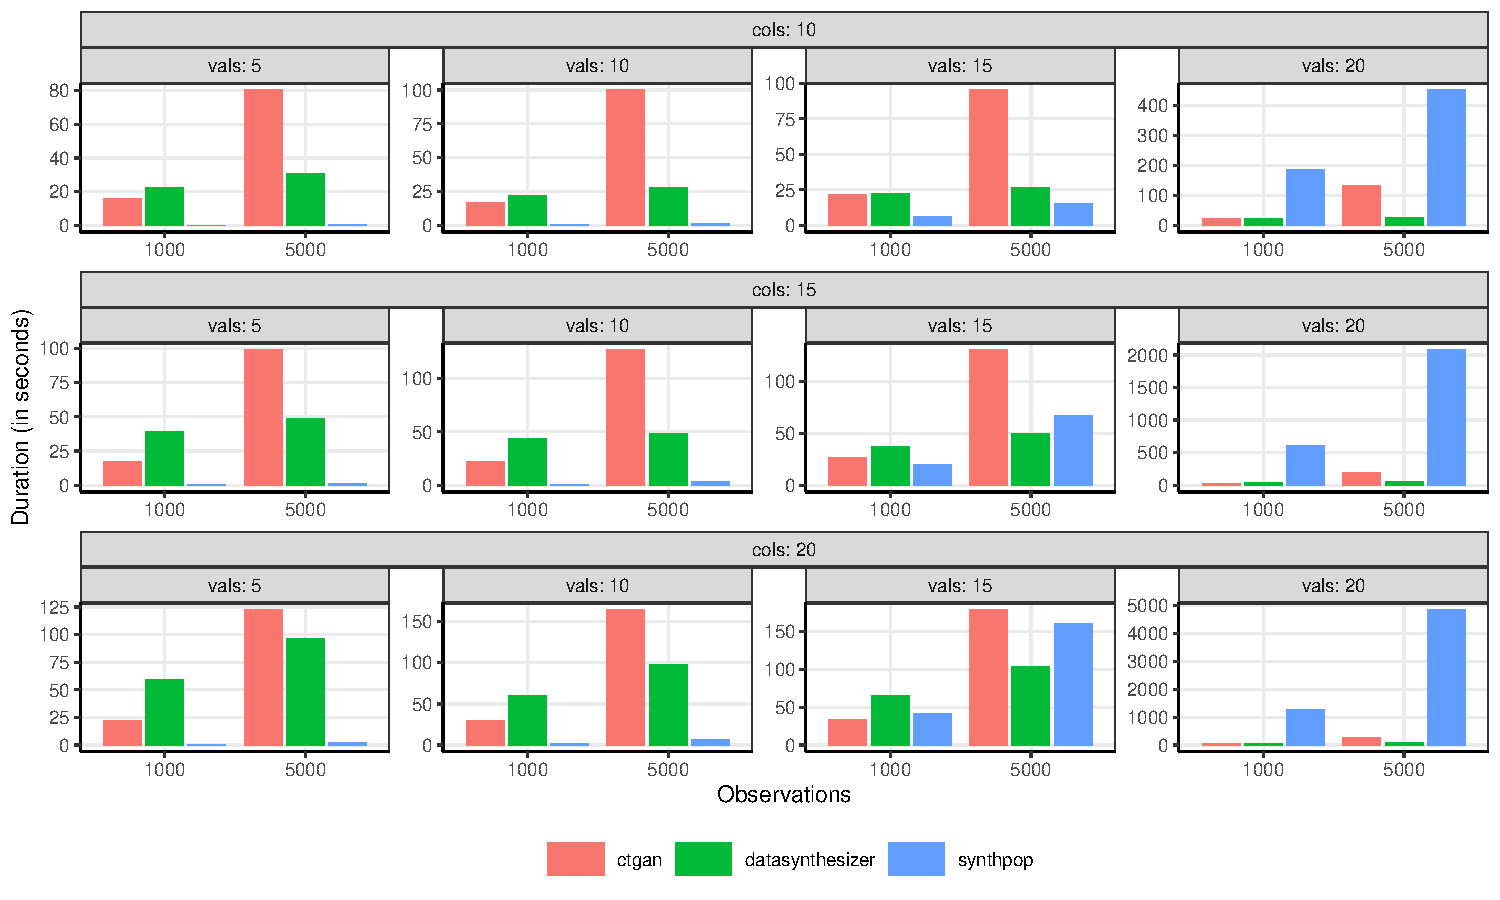
\includegraphics{../data/categorical_dim/graphs/graph_compare_duration.pdf}}
    \label{}
\end{figure}
}

\frame{\frametitle{Continuous data}
\tiny
CTGAN $=<$ Synthpop if (cols $>=$ 15 $|$ rows $>=$ 200.000) \\
Datasynthesizer always the best
\begin{figure}
    \caption{}
    \resizebox{.8\textwidth}{!}{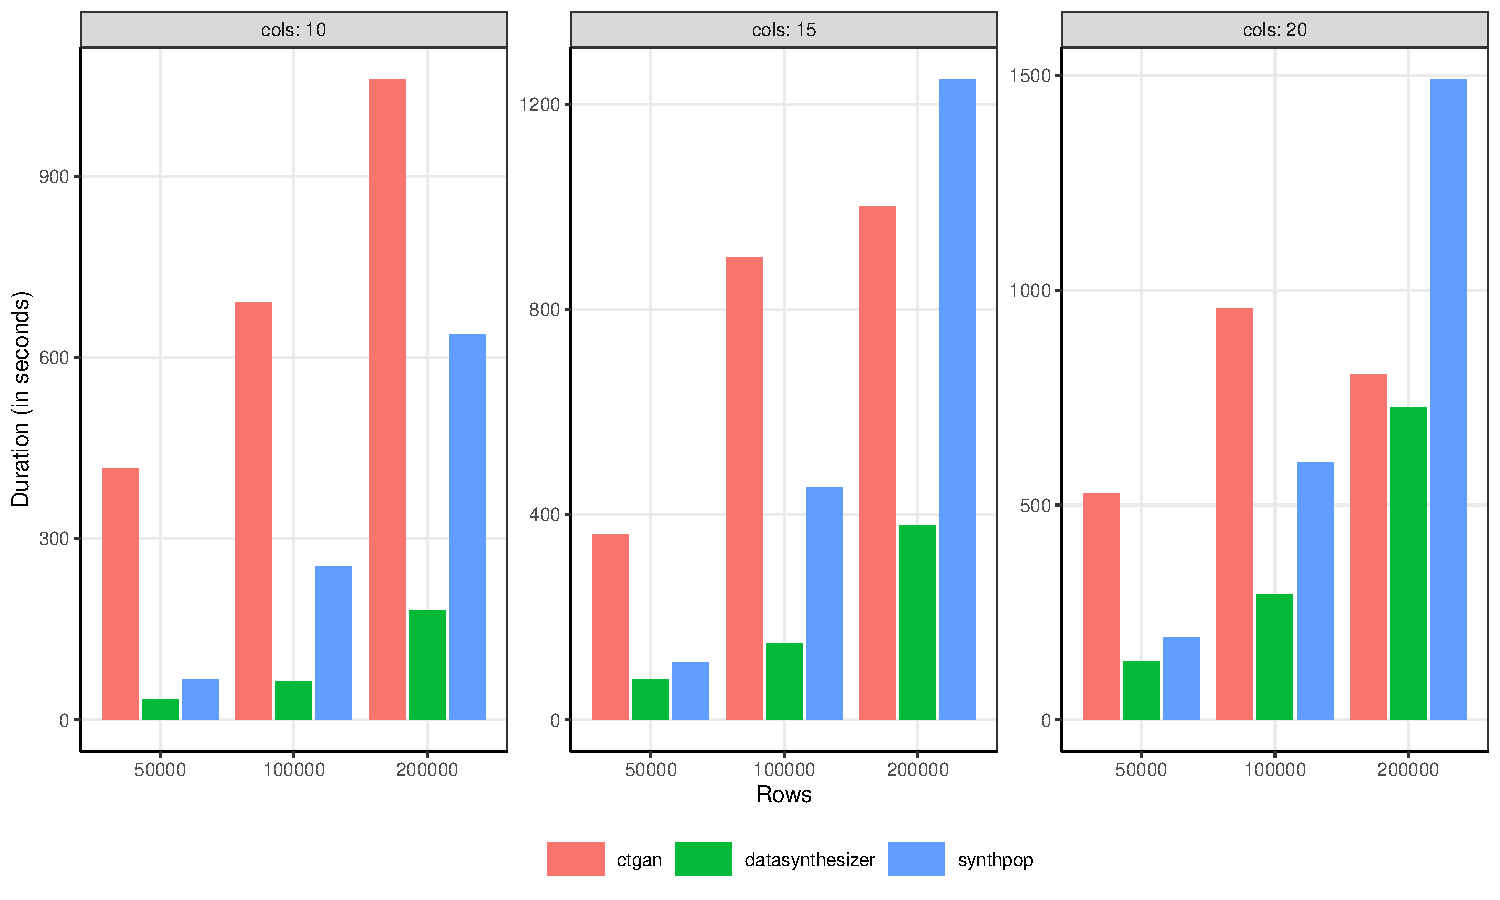
\includegraphics{../data/continuous_dim/graphs/graph_compare_duration.pdf}}
    \label{}
\end{figure}
\tiny{Note: CTGAN hyperparameter: batch size = 1000 and epochs = 50 (see figure \ref{graph_compare_ctgan_specks})}
}

\frame{\frametitle{Benchmark data}
Synthpop always the best, except SD2011 (full size), which has 2x as many variables as adult, but 1/4th number of rows
\begin{figure}
    \caption{}
    \resizebox{\textwidth}{!}{\includegraphics{../data/benchmark/graphs/graph_compare_duration.pdf}}
    \label{}
\end{figure}
}

\frame{\frametitle{Summary of efficiency}
\begin{itemize}
    \item Synthpop is fastest in low dimensional data
    \item It does not take very high levels of dimensionality for CTGAN/Datasynthesizer to be faster
    \item In high dimensional data, datasynthesizer $>$ CTGAN
\end{itemize}
}


%%%%%%%%%%%%%%%%%%%%%%%%%%%%%%%%%%%%%%%%%%
%%%%%%%%%%%%%%%%%%%%%%%%%%%%%%%%%%%%%%%%%%
%%%%%%%%%%%%%%%%%%%%%%%%%%%%%%%%%%%%%%%%%%
%%%%%%%%%%%%%%%%%%%%%%%%%%%%%%%%%%%%%%%%%%

\frame[c]{\frametitle{}
CTGAN vs. GANs 
}


\section{GANs}\label{sec:gans}
\frame{\frametitle{}
\begin{figure}
    \caption{Duration (CTGAN) w/continuous data}
    \resizebox{\textwidth}{!}{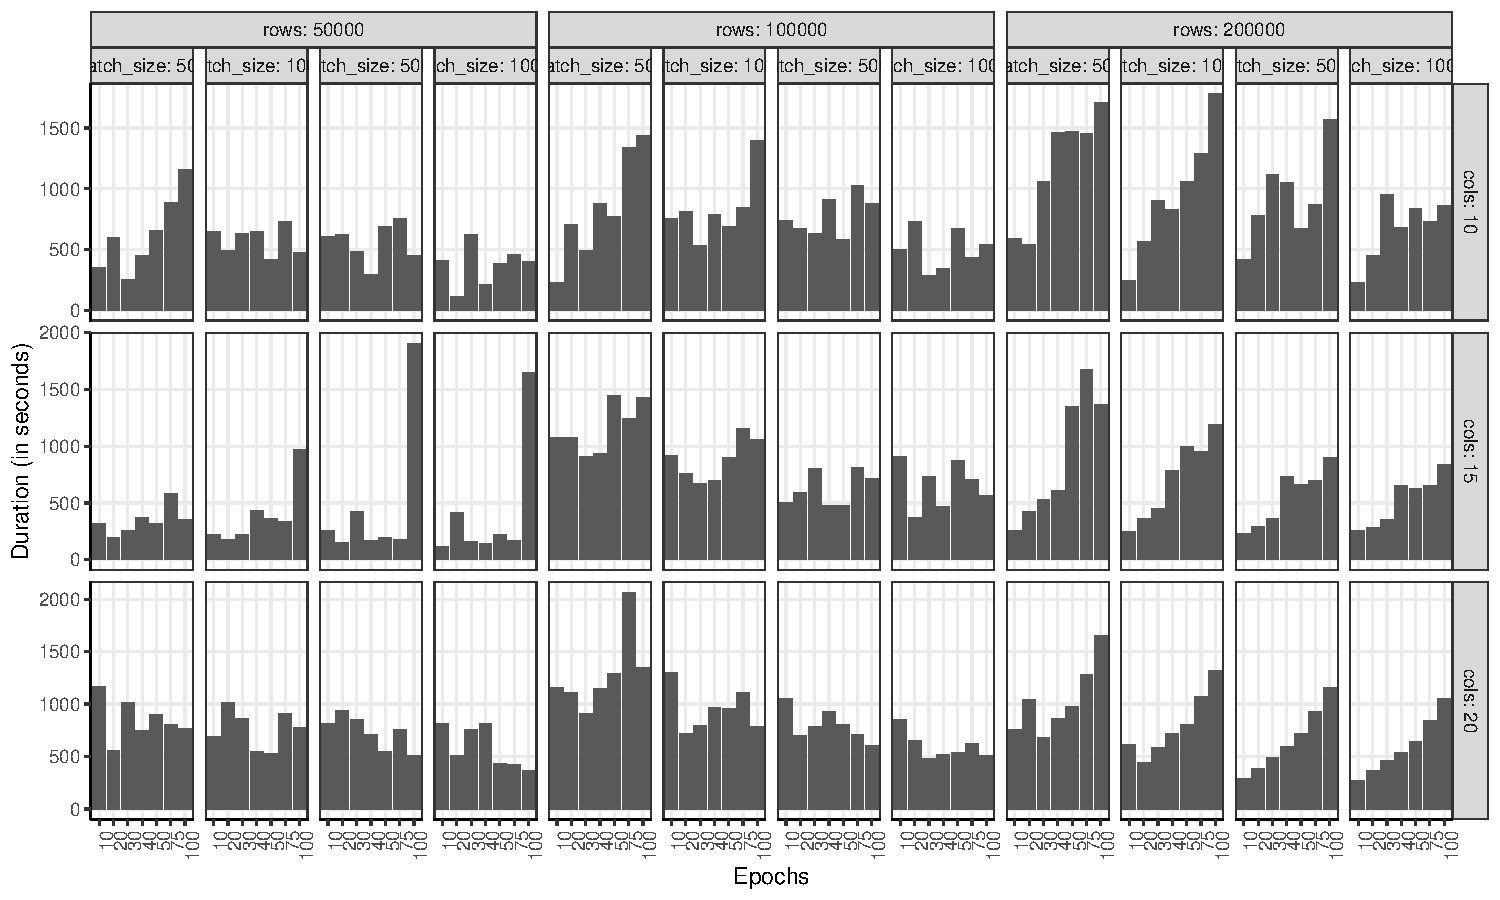
\includegraphics{../data/continuous_dim/graphs/graph_compare_ctgan_duration.pdf}}
    \label{}
\end{figure}
}

\frame{\frametitle{}
\begin{figure}
    \caption{Kolmogorov-Smirnov utility measure (CTGAN)}
    \resizebox{\textwidth}{!}{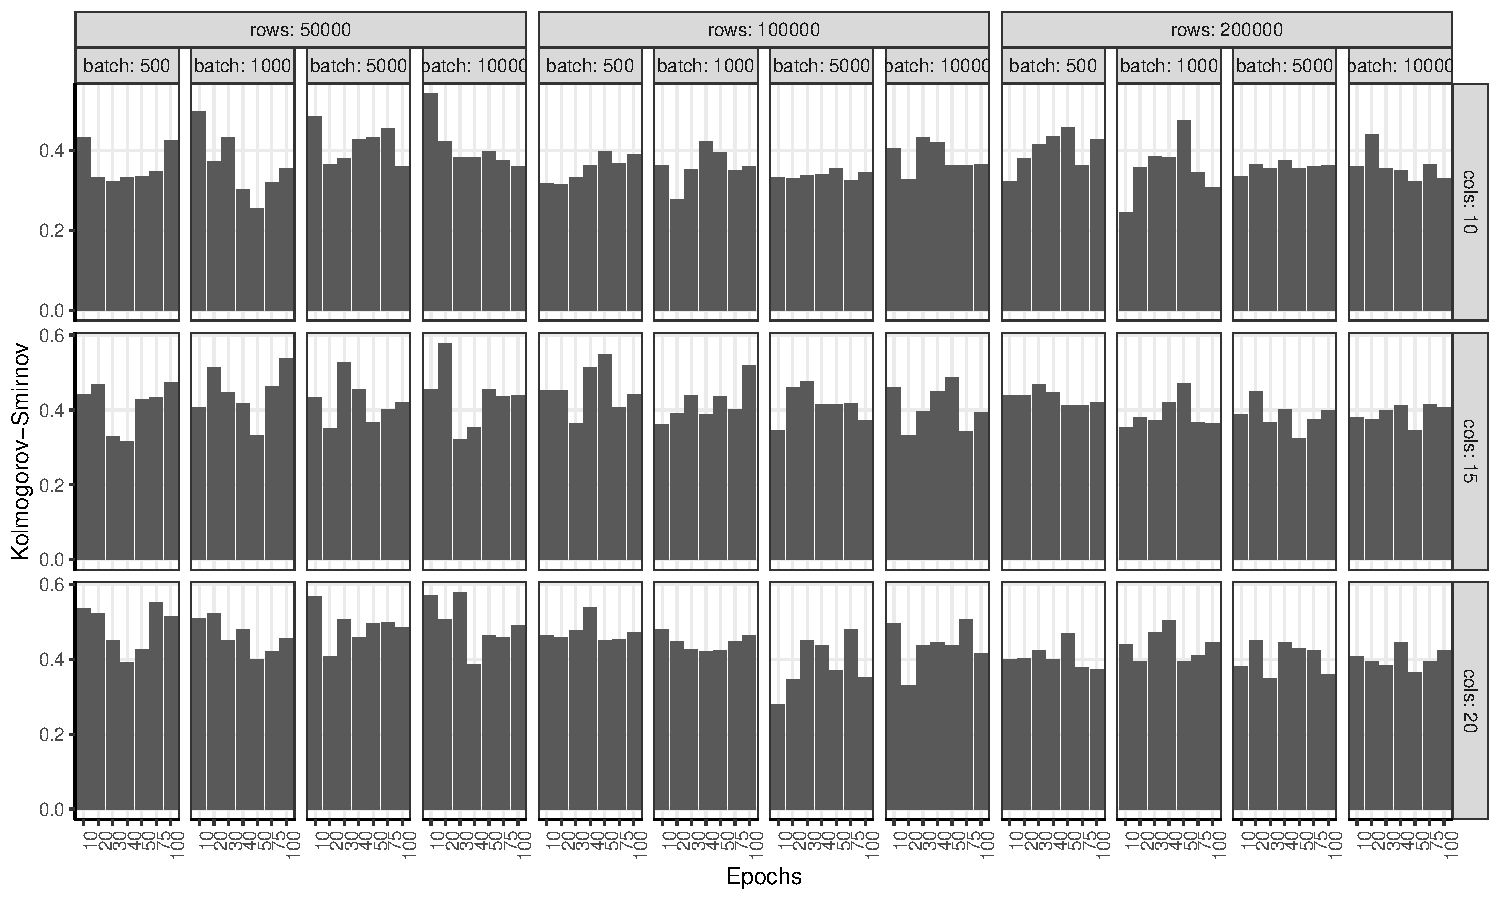
\includegraphics{../data/continuous_dim/graphs/graph_compare_ctgan_specks.pdf}}
    \label{graph_compare_ctgan_specks}
\end{figure}
}

\frame{\frametitle{Summary of GANs}
\begin{itemize}
    \item In CTAN, baseline is 300 epochs
    \item In single table, utility does not really change/improve after 50 epochs
    \item Utility of CTGAN is still worse than Datasynthesizer/Synthpop
    \item Can we create a better GAN?
    \begin{itemize}
        \item answer: yes we can (Neuenhoffer)
    \end{itemize}
\end{itemize}
}

%%%%%%%%%%%%%%%%%%%%%%%%%%%%%%%%%%%%%%%%%%
%%%%%%%%%%%%%%%%%%%%%%%%%%%%%%%%%%%%%%%%%%
%%%%%%%%%%%%%%%%%%%%%%%%%%%%%%%%%%%%%%%%%%
%%%%%%%%%%%%%%%%%%%%%%%%%%%%%%%%%%%%%%%%%%
\section{Synthpop}\label{sec:synthpop}

\frame[c]{\frametitle{}
Synthpop vs. cart
}

\frame{\frametitle{Methodology}
\footnotesize
\url{https://www.synthpop.org.uk/about-synthpop.html\#methodology}

Consider as an example a default synthesis, i.e. synthesis with all values of all variables (Y1, Y2,\dots, Yp) to be replaced. The first variable to be synthesised Y1 cannot have any predictors and therefore its synthetic values are generated by random sampling with replacement from its observed values. {\bf Then the distribution of Y2 conditional on Y1 is estimated and the synthetic values of Y2 are generated using the fitted model and the synthesised values of Y1.} Next the distribution of Y3 conditional on Y1 and Y2 is estimated and used along with synthetic values of Y1 and Y2 to generate synthetic values of Y3 and so on. The distribution of the last variable Yp will be conditional on all other variables. Similar conditional specification approaches are used in most implementations of synthetic data generation. They are preferred to joint modelling not only because of the ease of implementation but also because of their flexibility to apply methods that take into account structural features of the data such as logical constraints or missing data patterns.}

\begin{frame}[fragile]
    \frametitle{Synthpop (syn.cart)}
    \url{https://rdrr.io/cran/synthpop/src/R/functions.syn.r}
    \begin{lstlisting}[language=R]
syn.cart <- function(y, x, xp, smoothing = "", proper = FALSE, 
                     minbucket = 5, cp = 1e-08, ...)
fit <- rpart(y ~ ., data = as.data.frame(cbind(y, x)), method = "anova",
                 minbucket = minbucket, cp = cp, ...)
# get leaf number for observed data
leafnr  <- floor(as.numeric(row.names(fit$frame[fit$where,])))
# replace yval with leaf number in order to predict later node number 
# rather than yval (mean y for observations classified to a leaf) 
fit$frame$yval <- as.numeric(row.names(fit$frame))
# predict leaf number
nodes       <- predict(object = fit, newdata = xp)

...

uniquenodes <- unique(nodes)
new  <- vector("numeric",nrow(xp))
    for (j in uniquenodes) {
      donors <- y[leafnr == j] # values of y in a leaf
      new[nodes == j] <- resample(donors, size = sum(nodes == j), replace = TRUE)
    }

    \end{lstlisting}
\end{frame}

\frame{\frametitle{Method and code may not be the same}
\footnotesize

The code appears to indicate that the synthetic sample is drawn from the observed data in a predicted leaf, rather than the predicted y value.

Is this different than the methodological description?

Does this violate the definition of synthetic data, described above?

{\bf The point (and question): High levels of utility in synthpop may be the result of code that implements the method in a way that is not consistent with the definition of synthetic data}

If true, then utility in Synthpop may be artificially high (which lowers the relative advantage to other data synthesizers)

More research is needed 
}


%%%%%%%%%%%%%%%%%%%%%%%%%%%%%%%%%%%%%%%%%%
%%%%%%%%%%%%%%%%%%%%%%%%%%%%%%%%%%%%%%%%%%
%%%%%%%%%%%%%%%%%%%%%%%%%%%%%%%%%%%%%%%%%%
%%%%%%%%%%%%%%%%%%%%%%%%%%%%%%%%%%%%%%%%%%
\section{Utility}\label{sec:utility}

\frame[c]{\frametitle{}
Utility by synthesizer and data type
}


\frame{\frametitle{Categorical data}
\begin{figure}
    \caption{}
    \resizebox{\textwidth}{!}{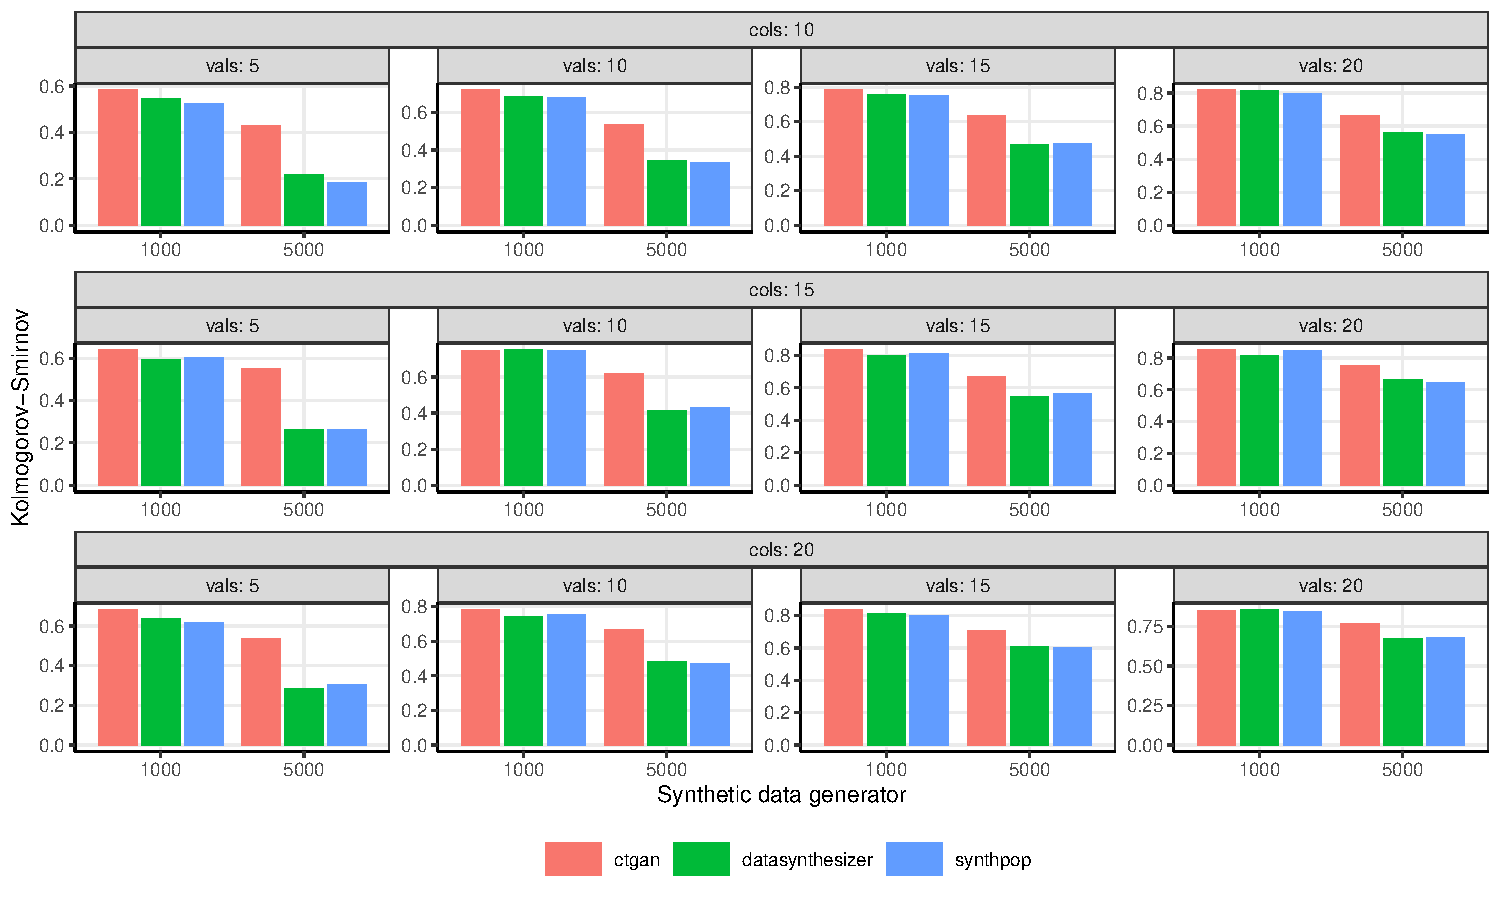
\includegraphics{../data/categorical_dim/graphs/graph_compare_utility_ks.pdf}}
    \label{}
\end{figure}
}

\frame{\frametitle{Continuous data}
\vskip -5mm
\begin{figure}
    \caption{}
    \resizebox{.9\textwidth}{!}{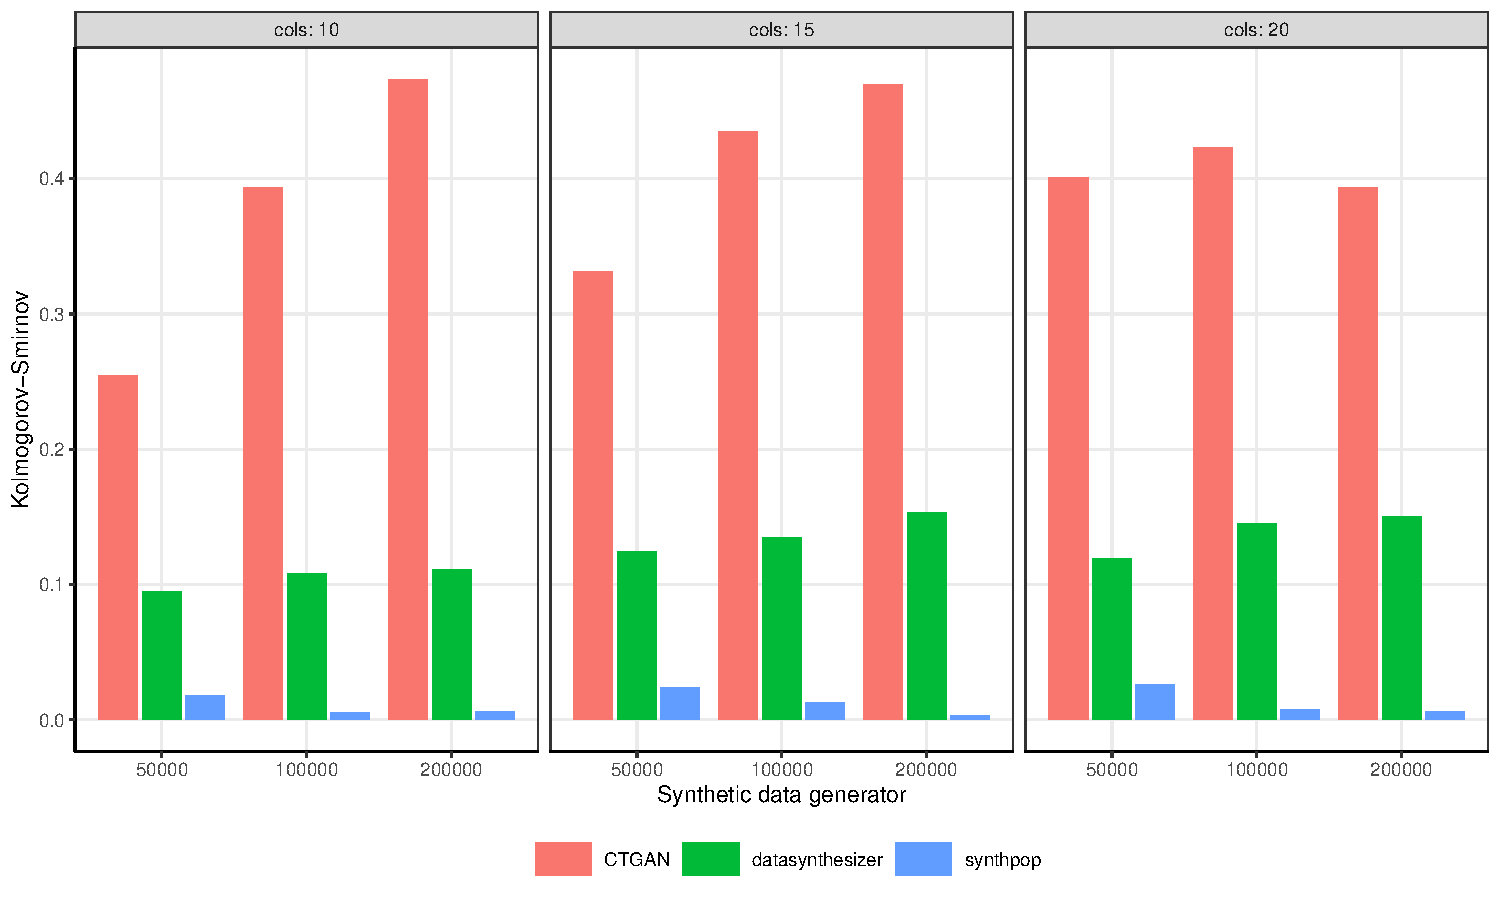
\includegraphics{../data/continuous_dim/graphs/graph_compare_utility_ks.pdf}}
    \label{}
\end{figure}
\tiny{Note: CTGAN hyperparameter: batch size = 1000 and epochs = 50 (see figure \ref{graph_compare_ctgan_specks})}
}

\frame{\frametitle{}
\begin{figure}
    \caption{Example frequency for continuous data with cols = 10}
    \resizebox{.9\textwidth}{!}{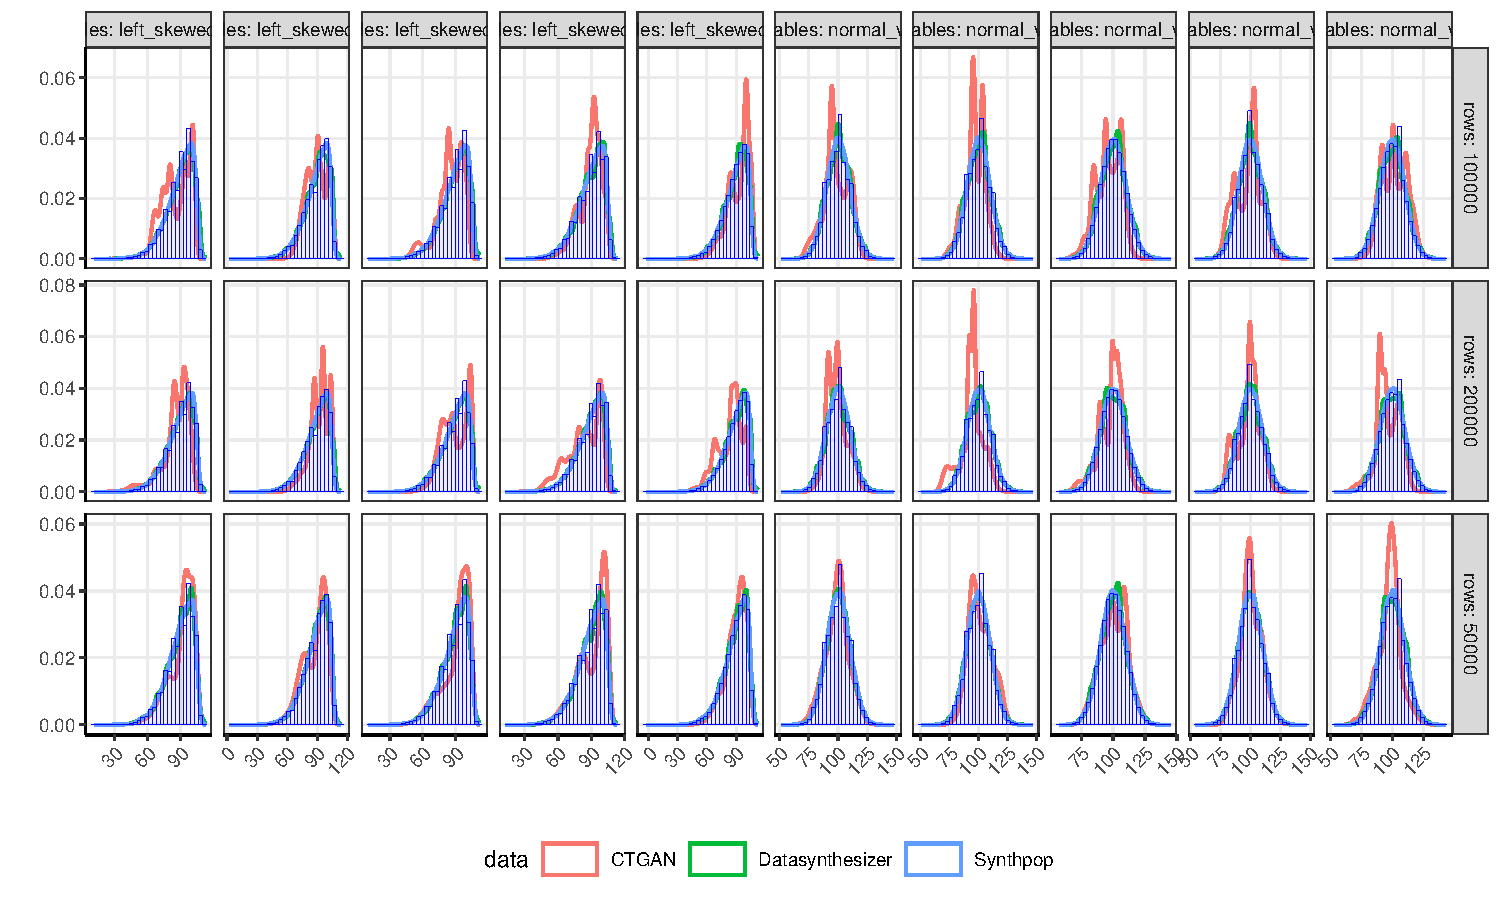
\includegraphics{../data/continuous_dim/graphs/graph_compare_frequency.pdf}}
    \label{}
\end{figure}
\tiny{Note: CTGAN hyperparameter: batch size = 1000 and epochs = 50 (see figure \ref{graph_compare_ctgan_specks})}
}

\frame{\frametitle{Benchmark data}
\begin{figure}
    \caption{}
    \resizebox{.9\textwidth}{!}{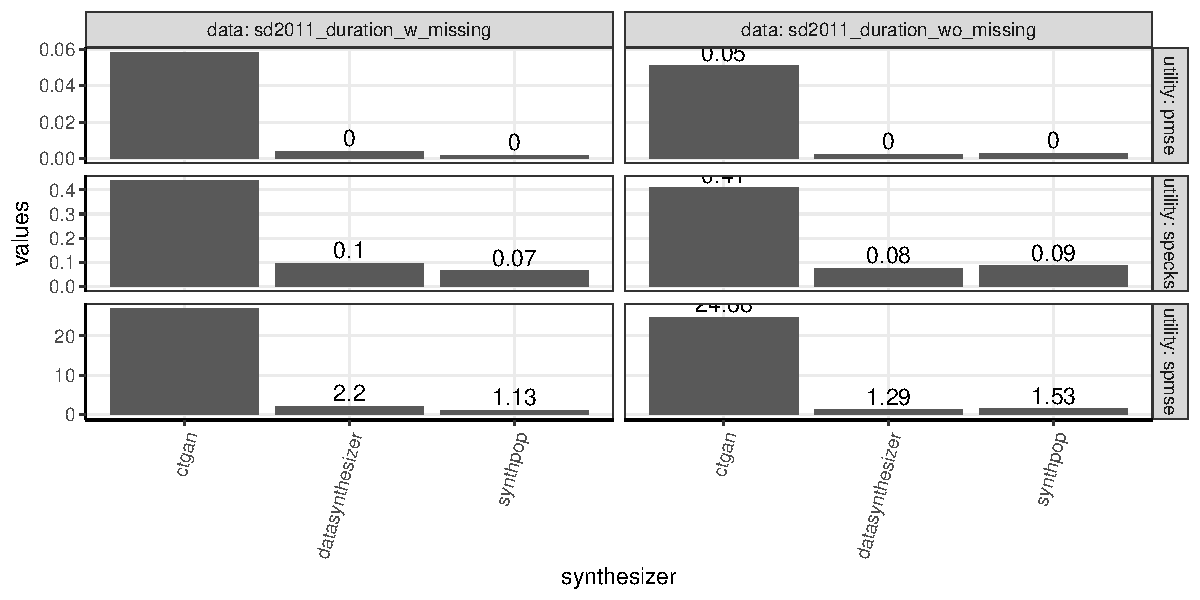
\includegraphics{../data/benchmark/graphs/graph_compare_utility.pdf}}
    \label{}
\end{figure}
}




\end{document}


